 \RequirePackage{docswitch}
% \flag is set by the user, through the makefile:
%    make note
%    make apj
% etc.
\setjournal{\flag}

\documentclass[\docopts]{\docclass}

% You could also define the document class directly
%\documentclass[]{emulateapj}

% Custom commands from LSST DESC, see texmf/styles/lsstdesc_macros.sty
\usepackage{lsstdesc_macros}

\usepackage{graphicx,subfigure}
\usepackage[titletoc]{appendix}
\usepackage{amsmath}
\usepackage{lineno}

%\usepackage{mathtools}
%\usepackage{subcaption} 
\graphicspath{{./}{./figures/}}
\bibliographystyle{apj}
\graphicspath{{figures/}}

% Add your own macros here:

\newcommand{\sne}{{SNe Ia }}
%\newcommand{\arcsec}{{$^{''}$}}
\newcommand{\pe}{{pe}}
\newcommand{\pesec}{{pe.s$^{-1}$}}
\newcommand{\phimax}{{$\Phi_{max}$}}
\newcommand{\opsim}{{\sc OpSim}}
\newcommand{\sncosmo}{{\sc SNCosmo}}
\newcommand{\redshift}{{$z$}}
\newcommand{\snstretch}{{$x_{1}$}}
\newcommand{\sncolor}{{$c$}}
\newcommand{\snx}{{$x_0$}}
\newcommand{\daymax}{{$t_{0}$}}
\newcommand{\degsq}{deg$^2$}
\newcommand{\colorerr}{{$\sigma_C$}}
\newcommand{\deltat}{{$\Delta_{t}$}}

\renewcommand\appendix{\par
  \setcounter{section}{0}
  \setcounter{subsection}{0}
  \setcounter{figure}{0}
  \setcounter{table}{0}
  \renewcommand\thesection{Appendix} %\Alph{section}}
  \renewcommand\thefigure{\Alph{section}\arabic{figure}}
  \renewcommand\thetable{\Alph{section}\arabic{table}}
}

\newcommand*\appendixwithtoc{{\bf \Huge Appendix}
  \cleardoublepage
  \appendix
  \addtocontents{toc}{\protect}%\StartAppendixEntries}
  %\listofatoc
}
% ======================================================================
\linenumbers
\begin{document}
\tableofcontents

\title{Snaps/no snaps: \\ saturation effects on supernovae in LSST}

\maketitlepre

\begin{abstract}

  Saturation phenomena occuring in all ccds affect flux measurements of nearby supernovae. A study to assess impacts of four parameters - point-like source flux, seeing (Point-Spread-Function), exposure time, and full well of the ccd - on supernovae light curve points is presented. Saturation effects up to z$\sim$ 0.05 for bright supernovae are observed and the $r$-band is the most affected. During the course of this study we have estimated reference curves (pixel flux distribution or saturated magnitudes as a function of the seeing) that could be used to include saturation effects in simulations. 

\end{abstract}

% Keywords are ignored in the LSST DESC Note style:
\dockeys{}

\maketitlepost

% ----------------------------------------------------------------------
% 

\section{Introduction}
\label{sec:intro}
While LSST observing strategy is not finalized yet, recent studies \cite{2018arXiv181200515L} have shown that it may be possible to observe a large sample of well-measured type Ia supernovae (\sne) up to a redshift of $z\sim 0.3-0.4$ in the Wide-Fast-Deep (WFD) survey. The main requirements on the cadence - typically few days for ($g,r,i$) bands with minimal inter-night gap variations - to achieve this result could be fulfilled by a rolling cadence strategy and/or by an optimized cadencing of the sky. The collection of few hundreds of thousands \sne (ie typically ten \sne~per square-degree) after ten years would open up unprecedented new perspectives in terms of supernovae cosmology, from anisotropy studies (Hubble diagram) to peculiar velocity measurements.\par
Very-low z ($z \lesssim 0.05$) \sne~are rare (about 1500 \sne~are expected to occur during 10 seasons of 180 days over 18000 \degsq) but quite luminous. The peak magnitude may be lower than 15 ($g$-band) for a typical \sne with $z\sim$ 0.01 which corresponds to a flux of more than 5.5 \textrm{$10^5$} photoelectrons (\pe) per second. The total number of photoelectrons collected with 15 s and 30 s exposures would be of 8.25 $ 10^{6}$ and 1.6 $ 10^{7}$ respectively.  These numbers exceed the expected full well capacity (90 ke) of LSST ccds. This would mean that, depending on the flux distribution over the pixels, some of \sne~fluxes may be unknown because of saturation effects. \par
We may identify four parameters impacting the total number of photoelectrons collected per exposure: the flux of the point-like source, the seeing (rules the flux distribution in the pixels), the full well capacity of the ccds (defines the saturation limit) and the time of exposure. In the current baseline ({\it snaps} scenario) LSST will take data as pairs of back-to-back, 15-second exposures to aid in cosmic-ray rejection. It may be possible to reduce overheads (by about 7\%) by moving to one exposure of 30s ({\it no snap} scenario). Other configurations (such as two snaps with distinct time of exposure like 10s-20s) could also be considered. In a recent report the LSST Science Advisory Commitee (SAC) has suggested use as default single 30-second exposures\footnote{This report is available at this url:https://project.lsst.org/groups/sac/meetings.}.\par

The purpose of this note is to study saturation effects on \sne~light curves. The first step involves estimating the flux distribution function as a function of the seeing for a set of Point Spread Function (PSF) models. The flux of a point-like source is spread over a set of pixels and the flux fraction of the pixel with the larger signal may be convolved with the telescope throughputs to evaluate magnitude corresponding to saturation (second step). The results depend on seeing, exposure time and full well of the ccd. Results obtained in the first part are applied to \sne~light curves in a third step. Impact of saturation is estimated using the flux distribution per band, the Signal-to-Noise Ratio of the measured fluxes and \colorerr, the error on the color parameter of \sne. Conclusions of this study are drawn in a last part. 

% ----------------------------------------------------------------------

\section{PSF and flux distribution function}
\label{sec:psfflux}
The flux fraction distribution of a point-like source depends on the following  parameters: pixel size (0.2$^{"}$ for LSST), PSF model, seeing and position of the center of the source in a pixel. The impact of the latter tend to decrease as the seeing increases. We have considered two PSF models:
\begin{itemize}
\item Single-gaussian profile:
  \begin{equation}
    \rho(r|\alpha)={\frac{1}{2\pi\alpha^2}}exp\left(-{\frac{r^2}{2\alpha^2}}\right) \label{eq:singlegauss}
   \end{equation}
\item Double-gaussian profile:
\begin{equation}
  \rho_K(r|\alpha)= 0.909 \left[\rho(r|\alpha)+0.1\rho(r|2\alpha)\right] \label{eq:doublegauss}
  \end{equation}
 \end{itemize}
Both satisfy the normalization requirement $ 2\pi \int^{\infty}_{0} \rho(r|\alpha) r dr = 1$ and FWHM=2.355$\alpha$. The second model \eqref{eq:doublegauss} corresponds to typically-observed seeing profiles and to those expected for Kolmogorov turbulence \cite{LSE40}. \par
We have simulated flux fraction distributions over square pixel maps ($\pm 3 \sigma$ around a central pixel corresponding to the position of the source) for a set of seeing (FWHM) values and for a map of source positions in the central pixel.  Two example of results are given on Fig.\ref{fig:fluxdist} for a seeing of 0.5\arcsec~ and a single gaussian PSF profile. Fig.\ref{fig:fluxpixels} displays the fraction of flux in each pixel for a source position in (0.,0.). As expected, the pixel in the middle contains the highest flux (around 13 to 14\% of the total flux in that case) and the flux distribution is symmetric.  Fig.\ref{fig:fluxposition} displays the fraction of flux in a pixel when the position of the source varies.The highest fraction is maximum (13 to 14\%) when the source position is in the middle of the pixel. Minimum values ($\sim$ 10 to 11\%) are obtained when the position of the source approaches the corners of the pixel.

\begin{figure}
  \subfigure[Flux distribution in pixels for a source position in (0.,0.).]{\label{fig:fluxpixels}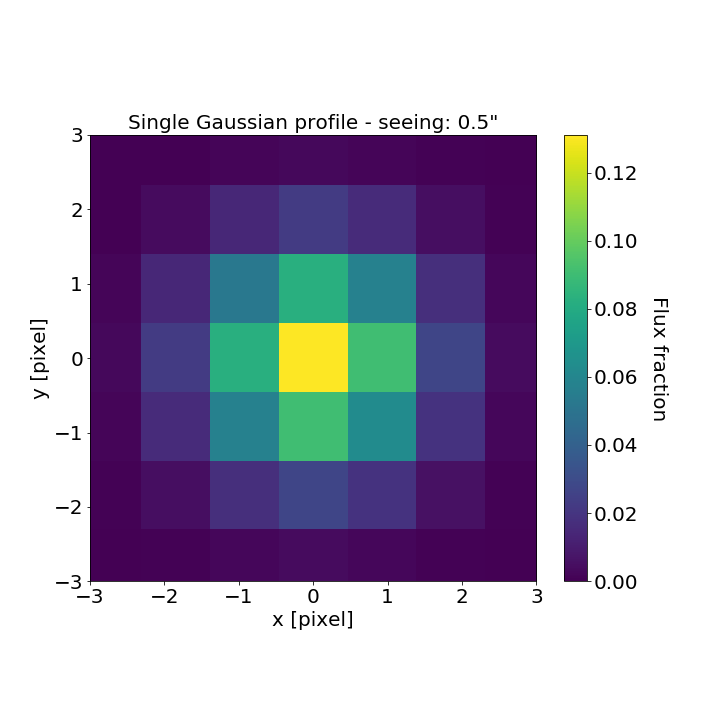
\includegraphics[width=0.5\textwidth]{flux_dist_seeing.png}}
  \subfigure[Fraction of flux of the central pixel as a function of the source position in this pixel.]{\label{fig:fluxposition}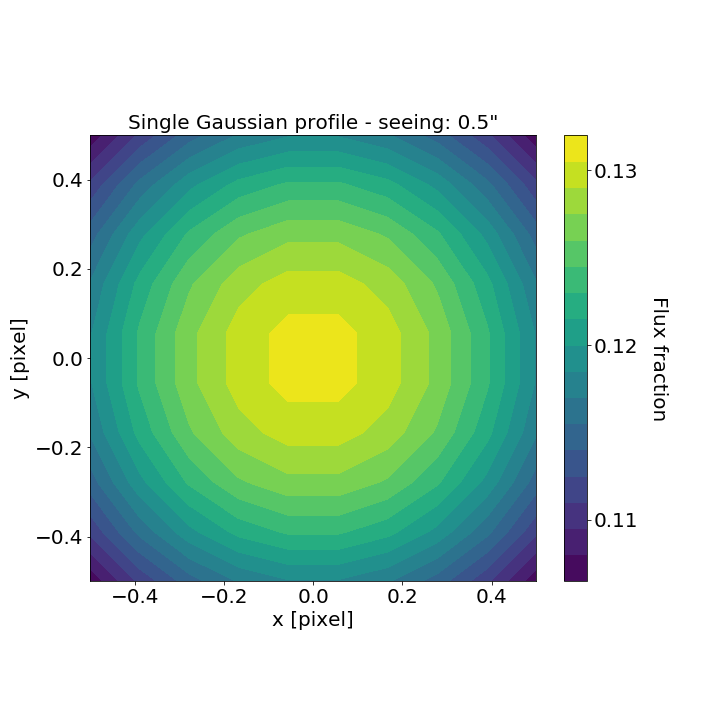
\includegraphics[width=0.5\textwidth]{flux_dist_center_position.png}}
  \caption{Flux distributions for a single gaussian PSF profile and a seeing of 0.5\arcsec.}\label{fig:fluxdist}
\end{figure}


A summary of the results obtained is given on Fig.\ref{fig:fracseeing} where the maximum fraction of flux in a pixel is displayed as a function of the seeing for a single gaussian (left) and a double gaussian (right) PSF profile. Highest fractions (typically 20 to 30\%) are reachable for seeing around 0.3\arcsec. The position of the source has a negligeable impact for seeings higher than 0.6\arcsec.
\begin{figure}[htbp]
\begin{center}
  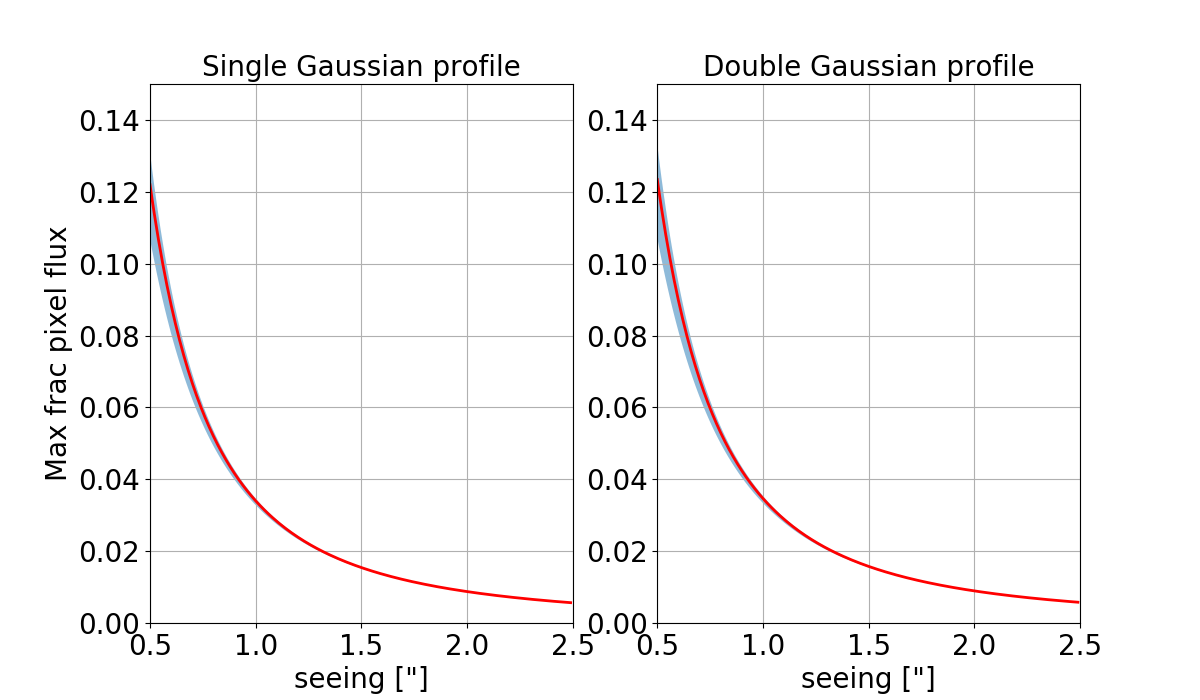
\includegraphics[width=0.9\textwidth]{max_frac_seeing.png}
 \caption{Maximum flux fraction (in a pixel) as a function of seeing for a single gaussian (left) and a double gaussian (right) PSF profile. The blue areas correspond to variations of the source position. Median values are represented by the red lines.}\label{fig:fracseeing}
\end{center}
\end{figure}

% ----------------------------------------------------------------------

\section{Saturated magnitude in LSST}
\label{sec:magsaturation}

It is possible to estimate the magnitude corresponding to pixel saturation by convolving  outcomes of Sect. \ref{sec:psfflux} with LSST intrument model. The method is the following:  magnitude is converted to photoelectrons using telescope throughput and exposure time; for a set of seeing values, results of Fig. \ref{fig:fracseeing} are used to estimate the highest number of photoelectrons in one pixel; saturation appears when the number of photoelectrons is greater or equal to full well capacity of LSST ccds. 

\begin{figure}[htbp]
\begin{center}
  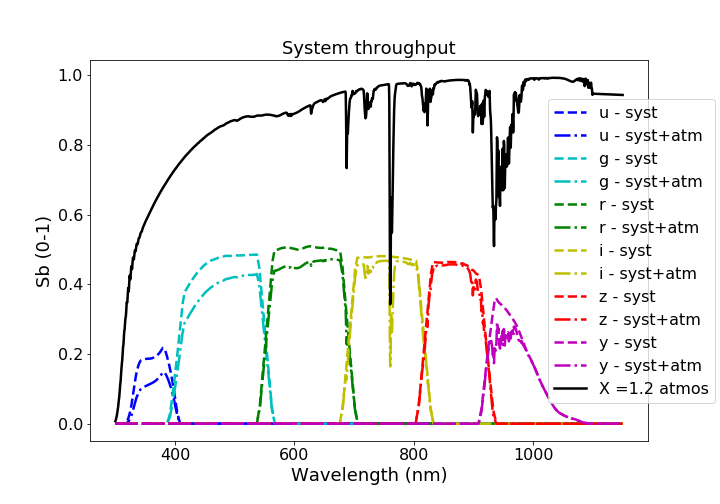
\includegraphics[width=0.6\textwidth]{LSST_throughput.png}
  \caption{LSST baseline throughput curves. Transmission (color) curves for LSST bands and for the telescope (syst: lens+mirrors+filters) with or without atmosphere transmission.  Effects of atmospheric transmission with an airmass value of 1.2 are illustrated by the black line.}\label{fig:throughput}
\end{center}
\end{figure}

\begin{figure}[htbp]
\begin{center}
  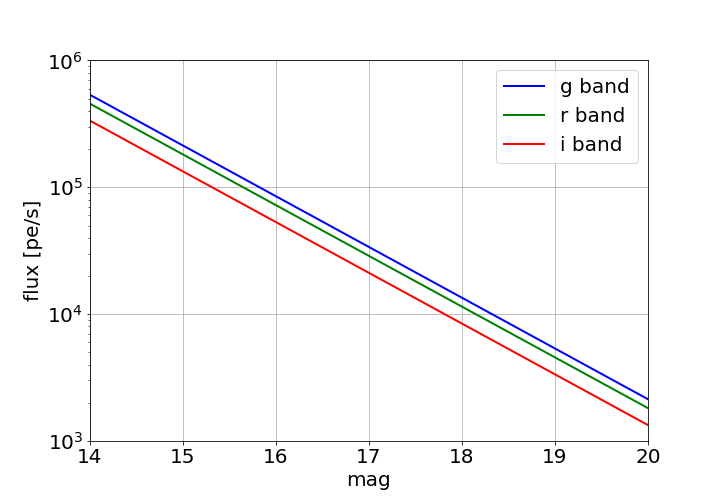
\includegraphics[width=0.6\textwidth]{flux_mag.png}
 \caption{Flux (in photoelectrons per second) as a function of magnitude for LSST throughput and airmass=1.2.}\label{fig:fluxmag}
\end{center}
\end{figure}

%\footnote{Files used to estimate these curves are available on github:https://github.com/lsst/throughputs/baseline}
LSST baseline throughput curves\footnote{Baseline curves are available in https://github.com/lsst/throughputs.} are given on Fig. \ref{fig:throughput}. These transmission curves can be used to estimate fluxes as a function of magnitude (Fig. \ref{fig:fluxmag}). Saturated magnitude as a function of the seeing are drawn on Fig. \ref{fig:magsat} for two exposure times (15 s and 30 s) and two full well capacities (90k \pe~and 120k \pe). As it could have been anticipated, highest saturated magnitude decrease with seeing values and cover the range [15.3,16.4], [15.2,16.2] and [14.8,15.9] for $g,r$ and $i$ bands, respectively, and for a typical seeing value of 0.8\arcsec. 
\begin{figure}[htbp]
%\begin{center}
 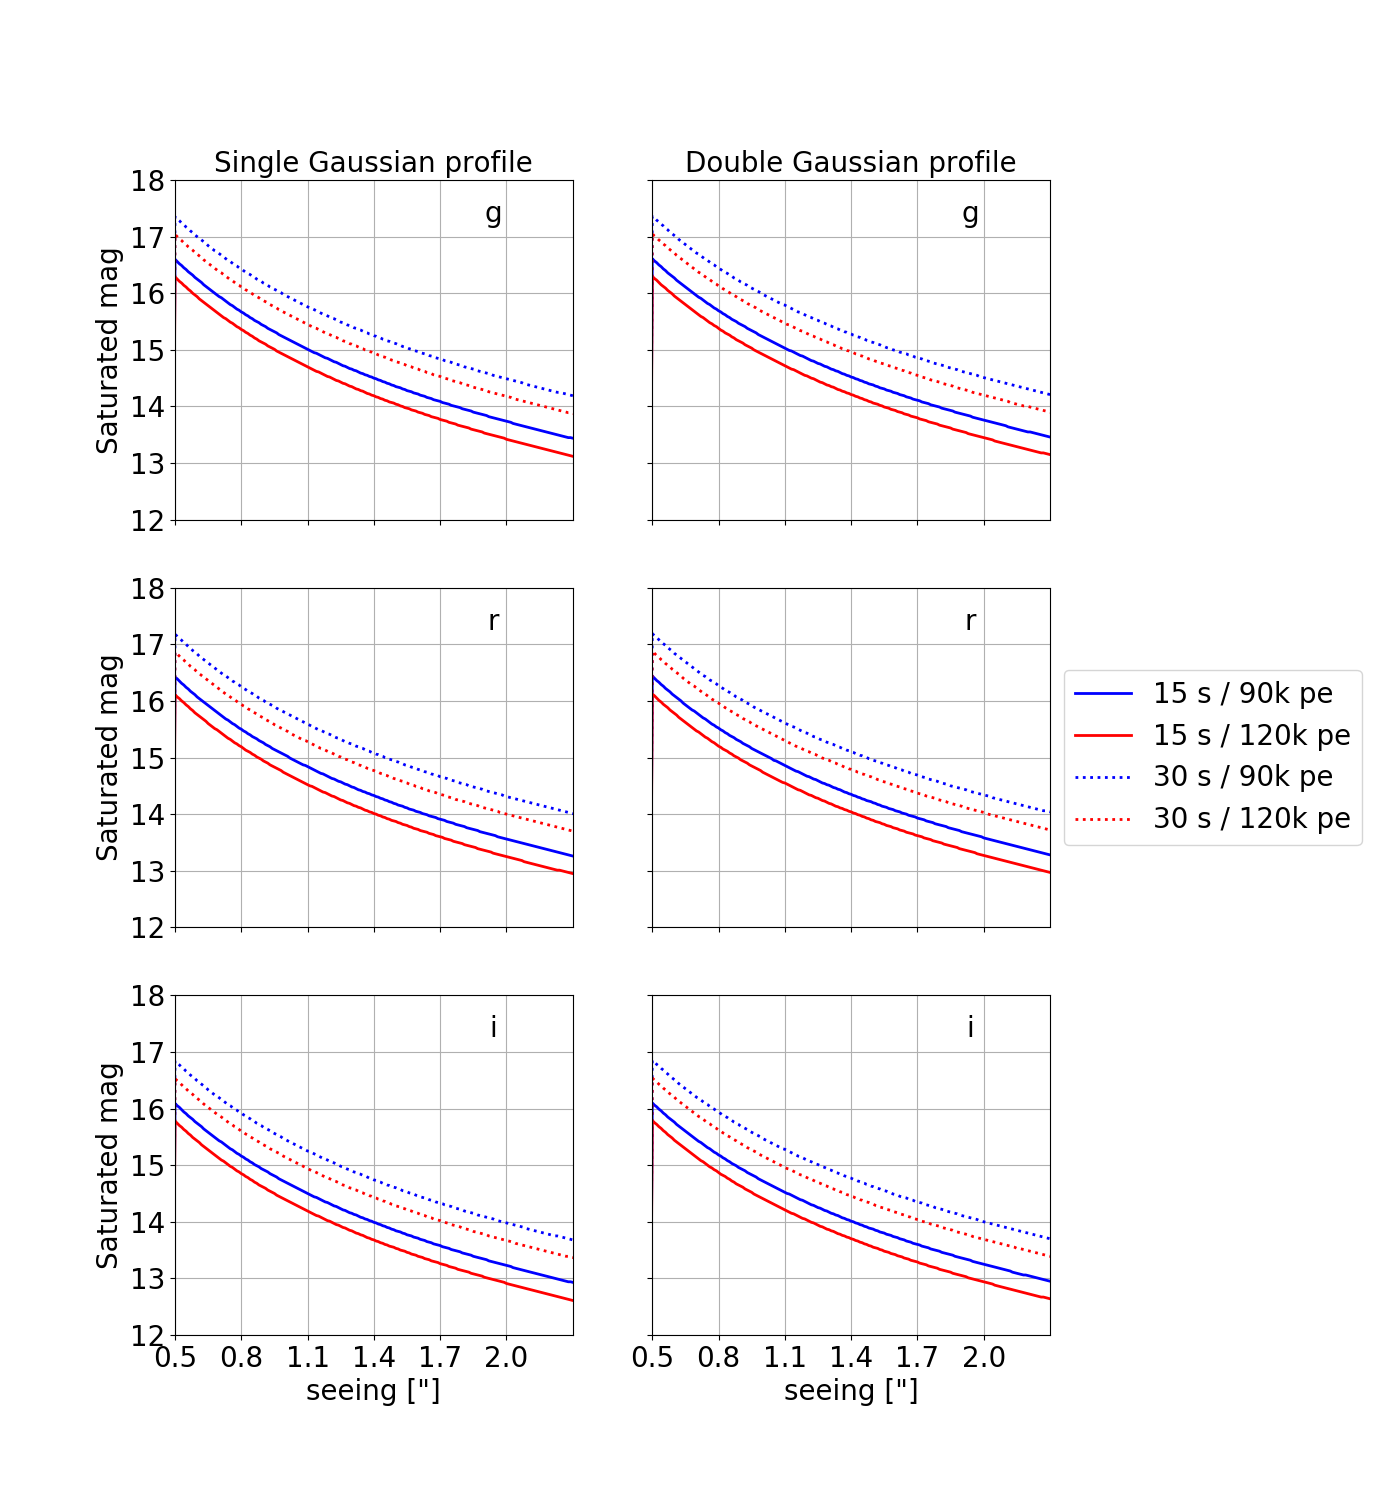
\includegraphics[width=1.1\textwidth]{magsat.png}
 \caption{Saturated magnitude as a function of seeing in LSST for $g, r$ and $i$ bands. Two exposure times (15 s: full line; 30 s: dotted line) and two full well capacities (90k \pe: blue; 120k \pe: red) have been considered.}\label{fig:magsat}
%\end{center}
\end{figure}

The relation between magnitudes for two configurations defined by two pairs (exposure time, full well) can be written:
\begin{equation}
\Delta m_{sat} = m^a_{sat}-m^b_{sat} = -2.5 \times \log\left(\frac{fw^a\times T_{exp}^b}{fw^b \times T_{exp}^a}\right)
 \end{equation}
where $fw$ is the full well capacity and $T_{exp}$ the exposure time. This relation is independent on the seeing and on the band. A comparison of the saturated magnitude is given on Tab. \ref{tab:satmagdiff}. The saturated magnitude increases by 0.75 if exposure time changes from 15 to 30s (full well: 90 \kpe). Increasing the full well to 120 k\pe allows to decrease the saturatd magnitude by 1.7. Balancing the increase in exposure time (from 15s to 30s) would request to double the full well value. 

\begin{table}[!htbp]
  \caption{Saturated magnitude difference wrt the default configuration (exposure time, full well) = (15s, 90 k\pe)}\label{tab:satmagdiff}
  \begin{center}
    \begin{tabular}{c|c|c}
      \hline
      \hline
      Exposure time (s) & full well (k\pe) & $\Delta m_{sat} $\\
      \hline
      \hline
      15  & 90 & -0.31\\
      30 & 90 & +0.75\\
      30 & 120 & +0.44\\
      \hline
    \end{tabular}
  \end{center}
  \end{table}

% ----------------------------------------------------------------------

\section{Impact of saturation on type Ia supernovae light curves}
\label{sec:sn_saturation}
Assessing saturation effects on type Ia supernovae simulated light curves involves evaluating, for each single LC points, the highest value of the flux (\phimax) deposited in a pixel. Saturation occurs (meaning that the flux is unknown and that the corresponding LC points can not be used) when \phimax~exceeds the full well capacity of this pixel. We have used simulated distributions of the seeing parameters to remove saturated LC points of a set of supernovae simulated light curves. Three metrics are used to assess staturation effects: flux fraction in each band, Signal-to-Noise Ratio (SNR) of the light curves (per band) and the error on the color parameter \colorerr.

\subsection{Seeing distributions}

Seeing distributions extracted from a simulation(the current observing strategy baseline kraken\_2026) performed with the LSST Operations Simulator(\opsim)\cite{2017arXiv170804058L} simulation are displayed on Fig. \ref{fig:seeing_opsim} for $ugrizy$ bands. Two types of seeings are available\footnote{These definitions are extracted from https://lsst-sims.github.io/sims\_ocs/tables/summaryallprops.html}:
\begin{itemize}
\item seeingFwhmGeom: “Geometrical” full-width at half-maximum, actual half width at maximum brightness. This can be used to represent the FWHM of a double Gaussian representing the physical width of a PSF.
\item seeingFwhmEff: “Effective” full-width at half-maximum, typically ~15\% larger than seeingFwhmGeom. This can be used to calculate SNR for point sources, using seeingFwhmEff as the FWHM of a single Gaussian describing the PSF.
\end{itemize}
The range of seeings varies from 0.5\arcsec~to 2.5\arcsec~with median values between 0.72\arcsec~and 0.97\arcsec (see Tab. \ref{tab:medseeing}).

\begin{table}[!htbp]
  \caption{Median seeing values from \opsim~run kraken\_2026.}\label{tab:medseeing}
  \begin{center}
    \begin{tabular}{lcccccc}
      \hline
      \hline
      band & u & g &r &i &z &y \\
      \hline
      \hline
      seeingFwhmGeom [\arcsec]  & 0.85 & 0.80 & 0.77 & 0.74 & 0.73 & 0.72 \\
      seeingFwhmEff [\arcsec] & 0.97 & 0.91 & 0.87 & 0.84 & 0.82 & 0.81 \\
      \hline
    \end{tabular}
  \end{center}
  \end{table}
      

\begin{figure}[htbp]
\begin{center}
  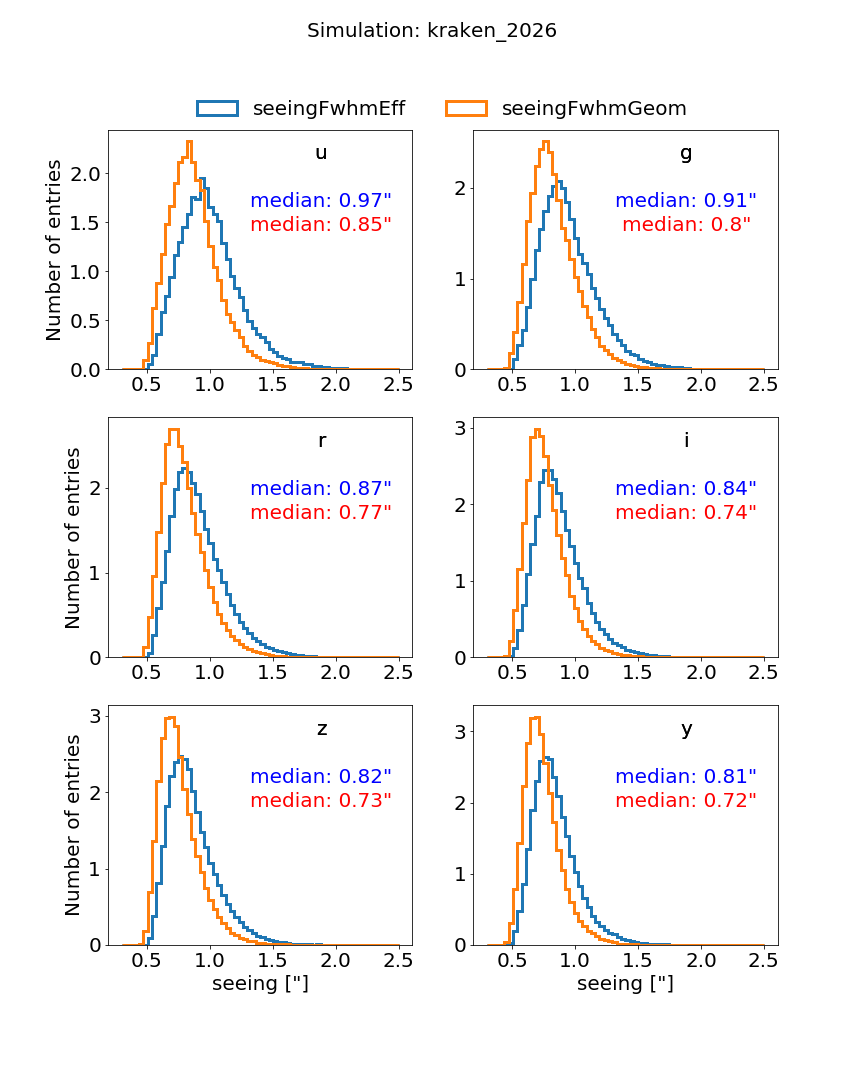
\includegraphics[width=0.9\textwidth]{seeing_kraken_2026.png}
 \caption{Seeing distributions extracted from \opsim~simulations dubbed as kraken\_2026.}\label{fig:seeing_opsim}
\end{center}
\end{figure}

\subsection{\sne light curve simulations}
Fluxes of type Ia supernovae have been simulated using \sncosmo~\cite{2016ascl.soft11017B}, a python library for supernova cosmology. Four parameters are used to define a supernova: the redshift \redshift, the stretch \snstretch, the color \sncolor, and the time-of-zero-phase \daymax. We have considered three cases in the (\snstretch,\sncolor) parameter space corresponding to:
\begin{itemize}
\item (\snstretch,\sncolor) = (-2.0,0.2) : faint supernova
\item (\snstretch,\sncolor) = (0.0,0.0) : medium supernova
 \item (\snstretch,\sncolor) = (2.0,-0.2) : bright supernova
\end{itemize}
Observing conditions (seeing and five-sigma depth) may have a non negligeable impact on LC points detections and correlations (seeing/five-sigma depth, and  seeing between observations) may be important. We have thus decided to use seeing and five-sigma depth distributions extracted from mean daily values (per band) from kraken\_2026.\par
We have simulated observations in $g,r,i$ bands with the following criteria:  regular cadence of three days (one measurement per band each day of observation shifted by ten minutes between bands); \daymax $\in$ [daymin+20*(1+z),daymax-40*(1+z)] (step: one day) where daymin(daymax)  stands for MJD of the first(last)  day of a year of observations (ten years have been simulated); $z~\in$[0.01,0.1] (step: 0.01); airmass equal to 1.2. \par
Two pairs of (exposure time, number of exposures) were considered: (15,2) and (30,1), corresponding to the {\it snaps} and {\it no snaps} scenarios, respectively. We have used LSST baseline throughput curves (Fig. \ref{fig:throughput}) to estimate the fluxes measured by the telescope.


Estimated magnitudes are given on Figs. \ref{fig:lcfaint},\ref{fig:lcmedium},\ref{fig:lcbright} for a faint, medium, and bright type Ia supernova, respectively. Minimal magnitudes are summarized in Tab. \ref{tab:minimag} and range from 14-15 (z$\sim$0.01, bright SN) up to $\sim$ 18 (z$\sim$0.05, faint SN). 

\begin{table}[!htbp]
  \caption{Minimal magnitudes as a function of redshift for faint, medium and bright type Ia supernovae.}\label{tab:minimag}
  \begin{center}
    \begin{tabular}{l|ccc|ccc|cccc}
      \hline
      \hline
      z        &\multicolumn{3}{c}{0.01} & \multicolumn{3}{c}{0.03} & \multicolumn{3}{c}{0.05} \\
      band & g & r & i & g & r & i & g & r &i \\
      \hline
      \hline
      faint SN   & 14.7 & 14.6 & 15.0 & 17.1 & 17.0 & 17.3 & 18.3 & 18.1 & 18.4 \\
      medium SN  & 14.0 & 14.0 & 14.6 & 16.3 & 16.4 & 16.9 & 17.4 & 17.5 & 18.0 \\
      bright SN & 13.2 & 13.5 & 14.2 & 15.5 & 15.9 & 16.5 & 16.6 & 17.0 & 17.6\\
      \hline
    \end{tabular}
  \end{center}
  \end{table}

Figure \ref{fig:method} illustrate the method we have adopted to study saturation impact on \sne~light curves. To every single simulated light curve point (in pe/sec - first row) corresponds a seeing (second row). According to the results exposed in Fig. \ref{fig:fracseeing} we estimate the highest fraction of energy deposited in a single pixel as a function of the seeing (third row). These factors are combined with the exposure time and  light curve points to estimate the highest signal (in pe) detected by a single pixel (fourth row). LC points with a flux higher than the chosen full well (here 90kpe) are not considered.\par
We could also have used  magnitudes of Fig. \ref{fig:magsat} to remove saturated LC points (seeing dependance). We have checked that both methods gave exactly the same results. 

\subsection{Saturation effects on \sne~light curves}

\subsubsection{Flux distribution per band}
Flux fraction (per band) of \sne~shows linear variations as a function of the redshift (Fig. \ref{fig:fluxmedium} for medium \sne, Figs. \ref{fig:fluxfaint} and ,\ref{fig:fluxbright} for faint and bright SN) and apportionnements between filters depend on the type (faint, medium, or bright) of the supernova. About 42\% of the flux of a faint \sne~is collected in the r-band, 31-34\% in the g-band, and about 25-27\%  in the $i$-band. $g$ and $r$ contributions are of the same order (about 40\%) for a medium \sne, with a fraction of flux in the $i$-band of 20-22\%.  $g$-band flux fraction is dominant for a bright \sne (about 47-49\%), followed by $r$-band ($\sim$ 37\%) and $i$-band (15-17\%) contributions.

Saturation effects are observed up to $z\sim$ 0.02, 0.03, and 0.05 for faint, medium, and bright \sne, respectively. Variations of flux distribution due to saturation may be quite complicated and depend on the type of \sne~and on the (exposure time,full well) configuration. Highest differences are observed at low redshifts (z$\sim$0.01-0.02) for the case (exposure time,full well)=(30s, 90k \pe) and for the bright \sne where $i$-band contribution dominates up to (z$\sim$0.025).

\begin{figure}[htbp]
\begin{center}
  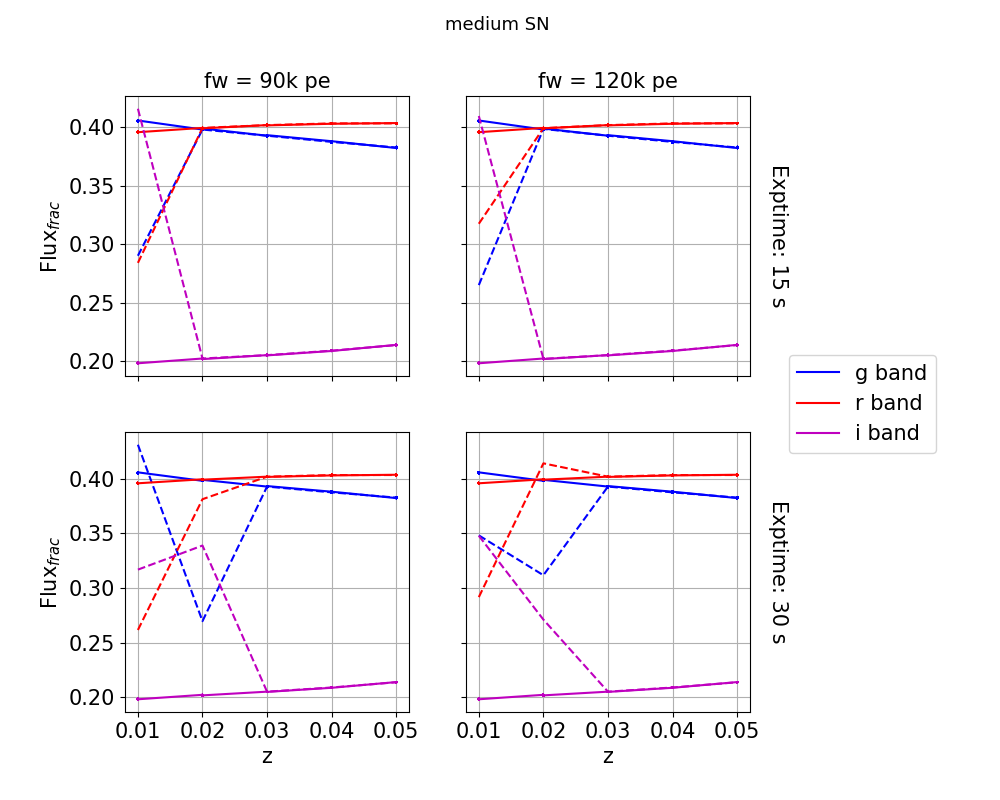
\includegraphics[width=0.9\textwidth]{Flux_medium.png}
 \caption{Saturation effect on flux distribution for a medium \sne. Flux fraction variations as a function of the redshift are given for $gri$ bands and four (exposure time, full well) configurations: (15s, 90k \pe) (top left),  (15s, 120k \pe) (top right), (30s, 90k \pe) (bottom left),  (30s, 120k \pe) (bottom right). All LC points have been considered to draw full lines. Dotted lines correspond to the case where saturated fluxes have been removed in the estimation (median values).}\label{fig:fluxmedium}
\end{center}
\end{figure}

\subsubsection{Signal-to-Noise Ratio}
The Signal-to-Noise Ratio is defined by band:
\begin{equation}
 SNR_{band} = \frac{\displaystyle \sum_{i=0}^{n}  \phi_{band}}{\sqrt{\displaystyle \sum_{i=0}^{n}  \sigma^2_{band}}}
\end{equation}
where the sums run over light curve points. (no SNR selection has been applied on these points). We have estimated SNR for the simulated light curve after application of the above-mentioned method to remove saturated points. We have normalized the results to the SNR estimated without saturation effects. 

\begin{figure}[htbp]
\begin{center}
  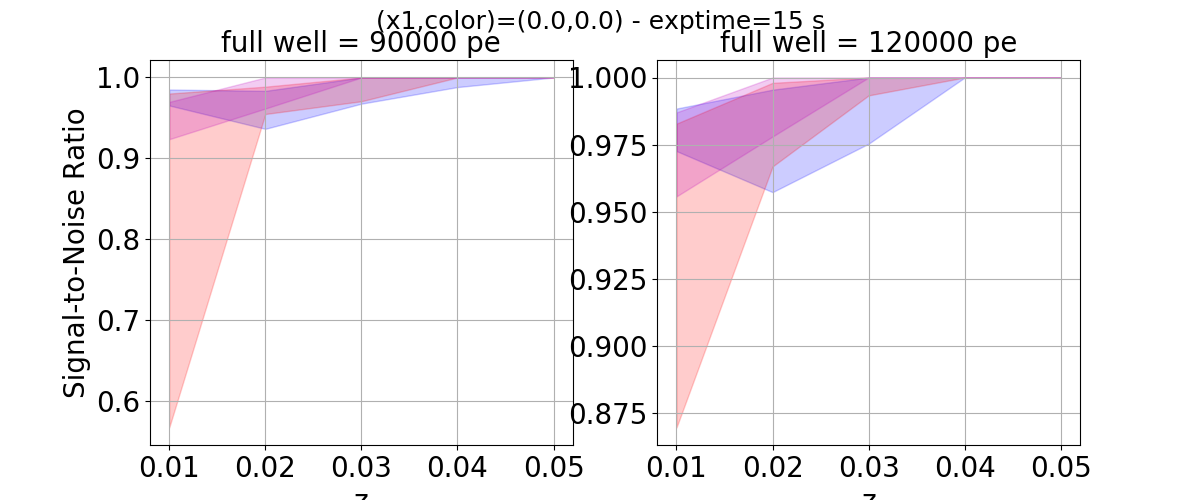
\includegraphics[width=0.9\textwidth]{SNR_medium.png}
 \caption{Saturation effect on Signal-to-Noise Ratio for a medium \sne. SNR (normalized to SNR values estimated without saturation included) variations as a function of the redshift are given for $gri$ bands and four (exposure time, full well) configurations: (15s, 90k \pe) (top left),  (15s, 120k \pe) (top right), (30s, 90k \pe) (bottom left),  (30s, 120k \pe) (bottom right).}\label{fig:snrmedium}
\end{center}
\end{figure}

Typical results for a medium supernova are displayed on Fig. \ref{fig:snrmedium} for four configurations in the (exposure time, full well) space parameters (results for faint and bright supernovae are on Figs. \ref{fig:snrfaint} and  \ref{fig:snrbright}, respectively). As expected highest variations occur for the (exposure time, full well)=(30s,90k \pe) scenario where SNR decrease of up to more than 40\% for z$\sim$ 0.01. 

\subsubsection{Time of saturation}

Early detection of supernovae is based on precise measurements of the rising light curves. Saturation effects degrade early detection (saturated LC points are not usefull for identification) and may be quantified by the difference in time \deltat~between the start of the LC rise (which we have identified as the time of the first LC point with $SNR \geq 5$) and the occurence of the first saturated LC point. The variation of  \deltat~as a function of the redshift is given on Fig. \ref{fig:deltatmedium} for a medium \sne. In the configuration (exposure time, full well) = (30s, 90 k\pe), saturation may occur in 5 to 6 days for $z ~0.01$.  \deltat~increases in a linear way as a function of redshift up to ~17.5 days for the $g$-band and $z~0.03$.

\begin{figure}[htbp]
\begin{center}
  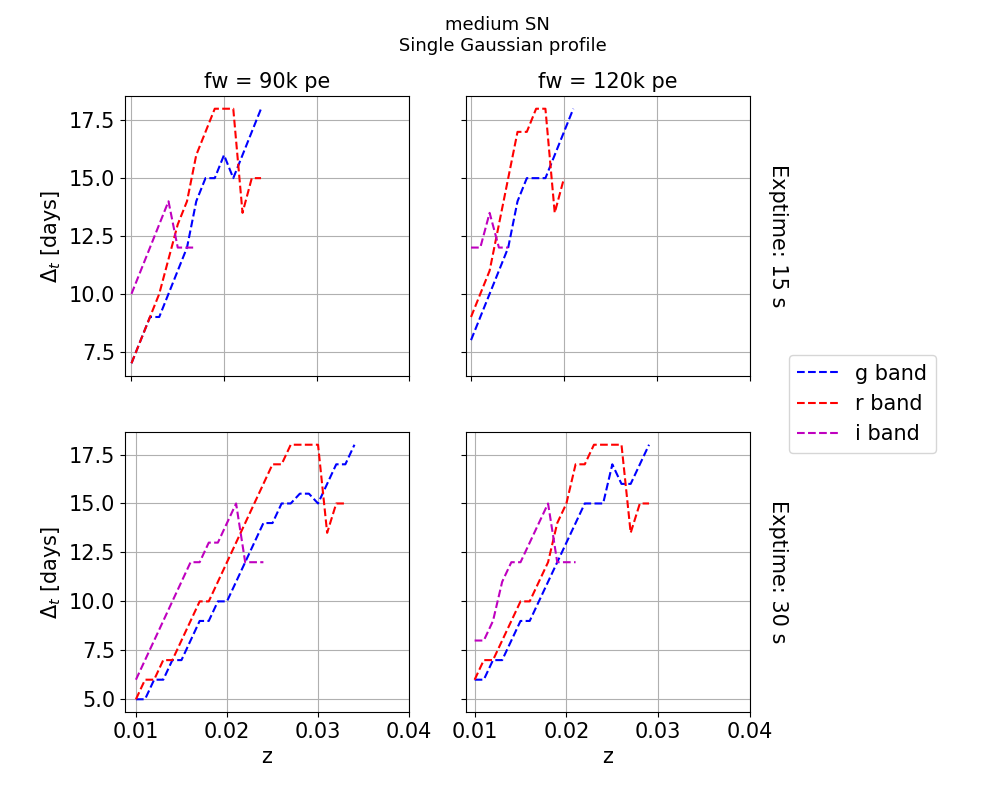
\includegraphics[width=0.9\textwidth]{DeltaT_medium.png}
 \caption{Saturation effect on \colorerr~for a medium \sne. \colorerr~variations as a function of the redshift are given for $gri$ bands and four (exposure time, full well) configurations: (15s, 90k \pe) (top left),  (15s, 120k \pe) (top right), (30s, 90k \pe) (bottom left),  (30s, 120k \pe) (bottom right). Dotted lines correspond to median values if LC saturated points are removed from \colorerr~estimation. Full lines correspond to the case where all LC points are considered (median values).}\label{fig:deltatmedium}
\end{center}
\end{figure}

\subsubsection{Distance modulus error}

A Hubble diagram
The assumption that supernovae with identical color, shape and galactic environment have on average the same intrinsic luminosity for all redshifts yields to  a standardized distance modulus:
\begin{equation}
  \mu =m_B*− M_B+\alpha \times \snstretch-\beta \times \sncolor)
\end{equation}
where $m_B^*$ corresponds to the observed peak magnitude in rest-frameB-band and $\alpha$,$\beta$ and $M_B$ are nuisance parameters. $\sigma_\mu$, the error on the distance modulus is evaluated  using \sne~parameter errors ($\sigma_\snstretch,\sigma_\sncolor,\sigma_{m_B}$) (estimated using Fisher formalism) with $\alpha$= 0.14 and $\beta=$ 3.1. 



\begin{figure}[htbp]
\begin{center}
  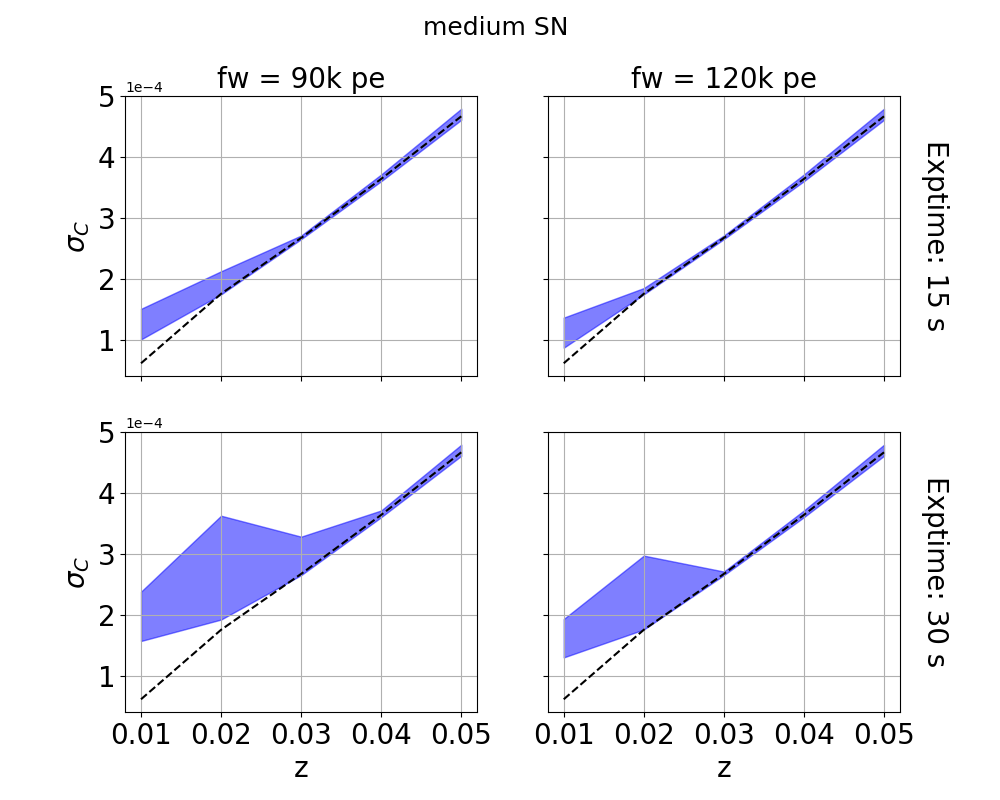
\includegraphics[width=0.9\textwidth]{sigmac_medium.png}
 \caption{Saturation effect on \colorerr~for a medium \sne. \colorerr~variations as a function of the redshift are given for $gri$ bands and four (exposure time, full well) configurations: (15s, 90k \pe) (top left),  (15s, 120k \pe) (top right), (30s, 90k \pe) (bottom left),  (30s, 120k \pe) (bottom right). Dotted lines correspond to median values if LC saturated points are removed from \colorerr~estimation. Full lines correspond to the case where all LC points are considered (median values).}\label{fig:sigmamedium}
\end{center}
\end{figure}


% ----------------------------------------------------------------------

\section{Conclusion}
\label{sec:conclusion}

In this document, we have studied impacts of four parameters (point-source flux, PSF, exposure time, ccd full well) to assess saturation effects on supernovae in LSST. Highest fractions of flux deposited in a pixel as a function of the seeing according to two PSF models (single gaussian and double gaussian profiles) were evaluated in a first stage. It was shown that pixels with highest fluxes collect $\sim$ 10\%, 5\%, and 3\% (median values) of the initial point-like source flux for seeing values of 0.5\arcsec, 0.8\arcsec, and 1\arcsec,  respectively.  These results have been convolved with LSST throughputs to estimate saturated magnitudes (per band) as a function of seeing, exposure time and ccd full well (second stage), leading to values in the range [15.4,16.4], [15.2,16.2] and [14.8,15.9] for $g,r$ and $i$ bands respectively, for seeing values of $\sim$ 0.8\arcsec. In a last stage we have estimated impacts of saturation on type Ia supernovae using three metrics - the flux distribution (per band), the Signal-to-Noise Ratio (par band), and \colorerr, the error of the color parameter - and a realistic simulation of light curves using \opsim~observing conditions. Effects have been observed up to $z\sim$ 0.02, 0.03 and 0.05 for faint, medium and bright supernovae, respectively.

During the course of this study we have estimated a set of reference curves\footnote{These curves are available at ...} (highest flux fraction in a pixel as a function of the seeing in stage 1, LSST saturated magnitudes -per band- as a function of the seeing in stage 2) that could be included in simulations of very-low $z$ \sne. 


% ----------------------------------------------------------------------

\subsection*{Acknowledgments}

%%% Here is where you should add your specific acknowledgments, remembering that some standard thanks will be added via the \code{desc-tex/ack/*.tex} and \code{contributions.tex} files.

%This paper has undergone internal review in the LSST Dark Energy Science Collaboration. % REQUIRED if true


 % Standard papers only: author contribution statements. For examples, see http://blogs.nature.com/nautilus/2007/11/post_12.html

% This work used TBD kindly provided by Not-A-DESC Member and benefitted from comments by Another Non-DESC person.

% Standard papers only: A.B.C. acknowledges support from grant 1234 from ...

\input{desc-tex/ack/standard} % also available: key standard_short

% This work used some telescope which is operated/funded by some agency or consortium or foundation ...

% We acknowledge the use of An-External-Tool-like-NED-or-ADS.

%{\it Facilities:} \facility{LSST}

% Include both collaboration papers and external citations:
\bibliography{main,lsstdesc}
\clearpage

\appendixwithtoc

\input appendix
\end{document}

% ======================================================================
